\section{Menu główne (Zofia Sosińska)}\label{chap:menu_main}
Przed startem właściwej gry, użytkownikowi ukazuje się menu główne. Pełni ono funkcję reprezentatywną, więc ważne było, aby współgrało ono z głównym programem.
Zgodnie z projektem udostępnia ono trzy kluczowe funkcjonalności:
rozpoczęcie nowej gry, wczytanie zapisanej oraz wyjście z programu.
Przycisk nowej gry
Po kliknięciu przycisku odczytu, pojawi się lista zapisów. Użytkownik może ją przeglądać, ruszając suwakiem po prawej stronie. Po naciśnięciu 


\begin{figure}[htbp]
    \centering
    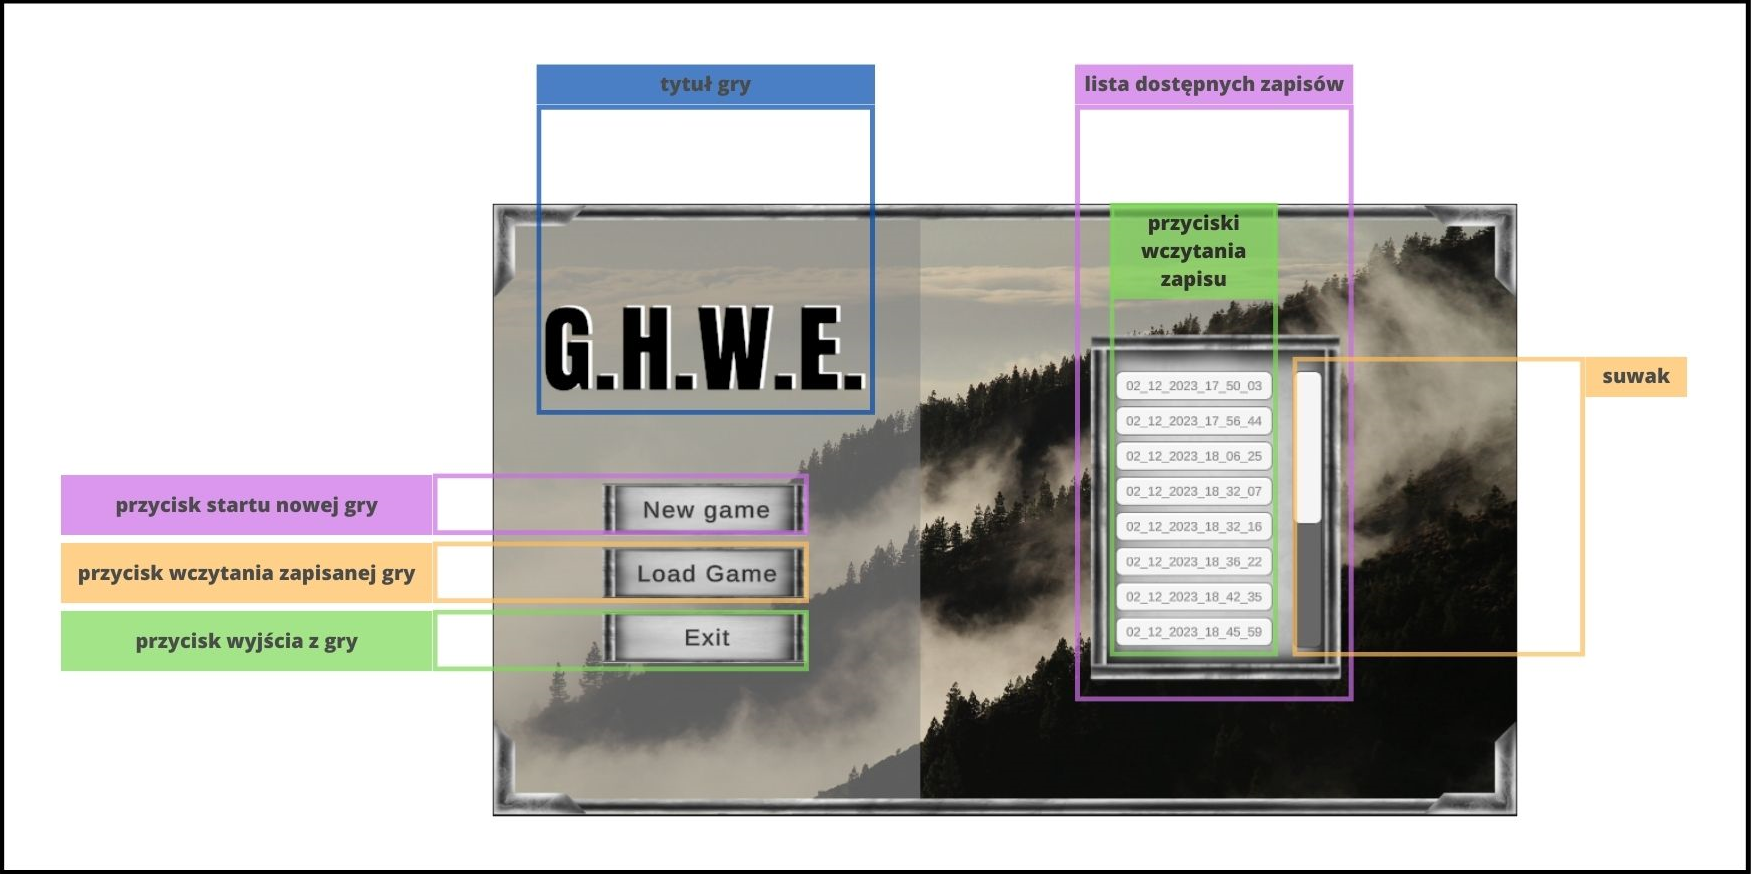
\includegraphics[width=0.9\textwidth]{images/ui/main_menu.png}
    \caption{Implementacja menu głównego.
    }\label{fig:compass}
\end{figure}